\chapter{Merchandise}

Merchandise at Venturer Camp 2023 was coordinated by Tom Brooks. The brief for merchandise was that it needed to represent Venturer Camp 2023, give attendees another Woodcraft T-Shirt which they could add to their collection and not loose money. A key factor here was that the main camp merchandise could not loose money as we had already planned to spend a lot on the Early Bird T-Shirts.

\section{What To Order}
The question of what merchandise to order is a question for the ages. Now that Woodcraft Folk uses \textit{Teemill} as it's online shop, rather than an in-house operation based out of Folk House - the logistics of selling un-sold merchandise gets more complex. In the end, it was decided to keep merchandise simple, offering:
\begin{itemize}
    \item Early Bird T-Shirt (for those who had booked \& paid in time to get one)
    \item Normal Camp T-Shirt (in 2 colours)
    \item Stickers with the Venturer Camp logo on
\end{itemize}
Additionally, ex-Folk Supply stock from Woodcraft Folk's old Crampton Street location was sold off. This had been in storage at Biblins since the closure of the old offices. Camp100 also provided a stock of t-shirts which the Venturer Camp merchandise stall sold to promote their event.

\section{What Got Sold}
The merchandise was very popular amongst attendees and it was felt that the pricing was reasonable. The t-shirts were priced at \pounds15 with other items being cheaper than this. \\

All the extra early-bird t-shirts were sold as well as over three quarters of the main camp t-shirts. Other items success varied, unfortunately we didn't gather data on the sales in the shop so we are unable to provide them here. \\

Any excess stock was transported to Cudham where it will be sold off and profits from which will go towards the centre.

\begin{figure}[ht]
    \centering
    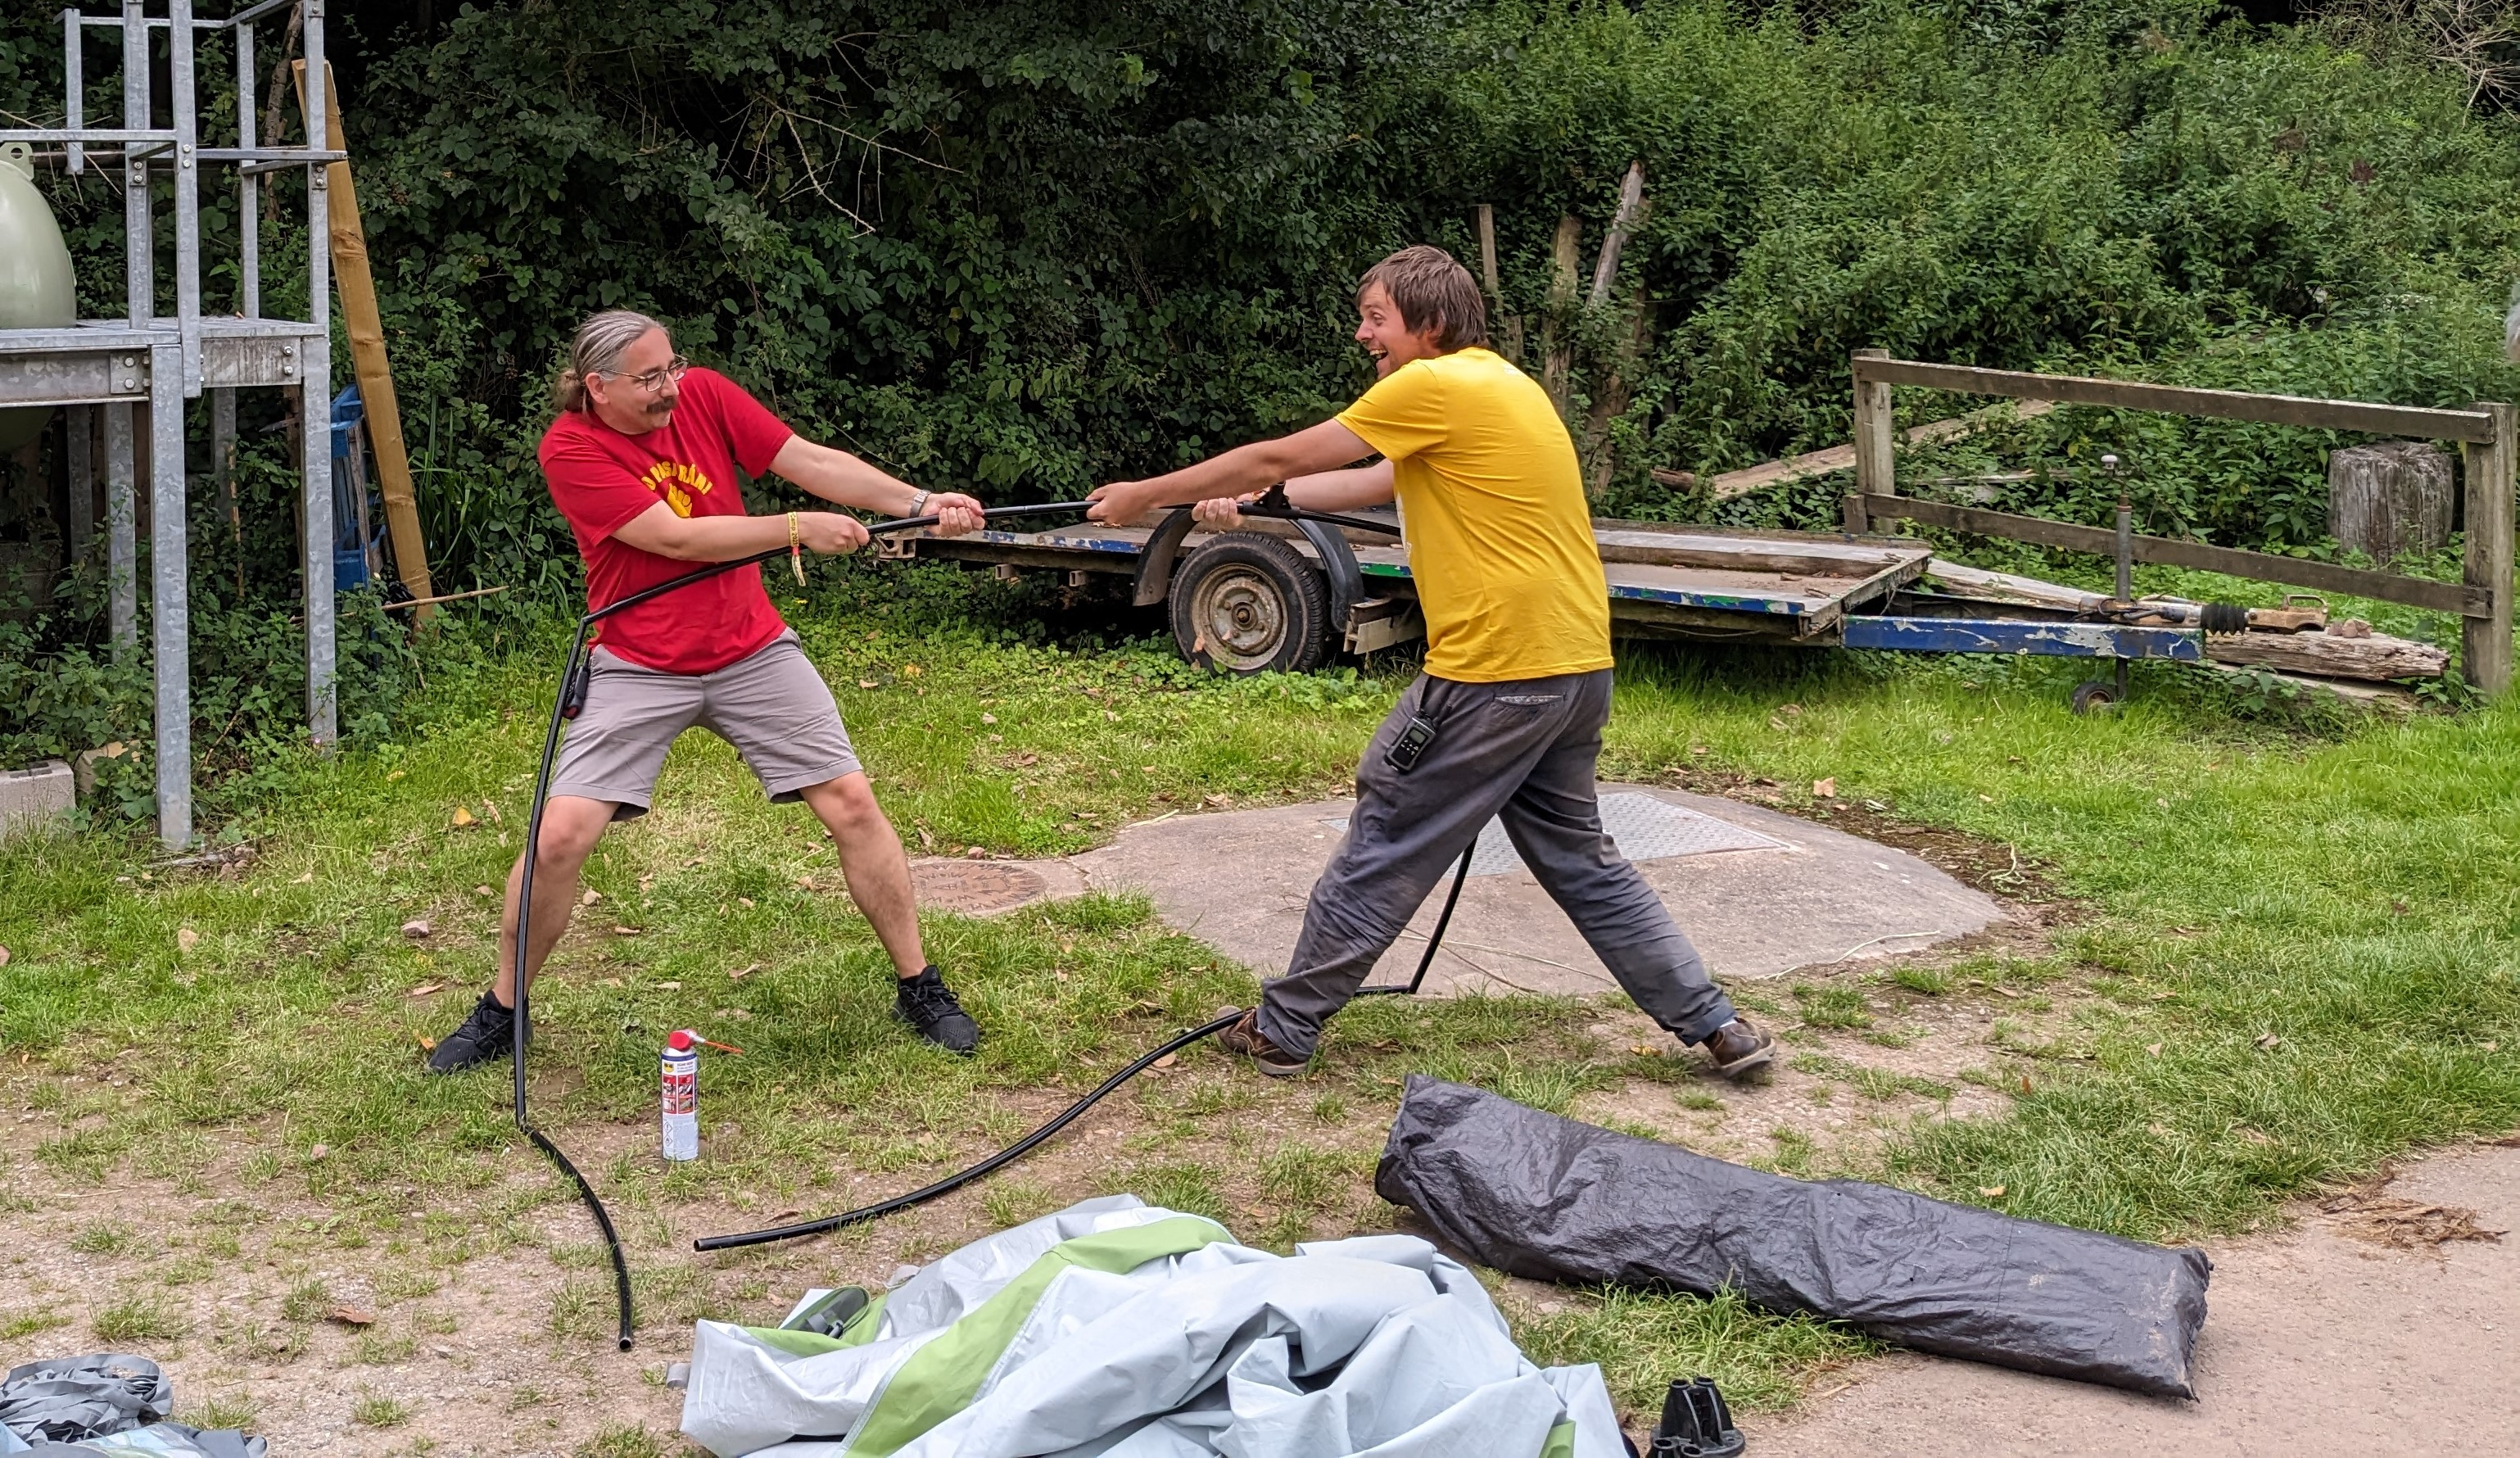
\includegraphics[width=0.8\textwidth]{assets/disassembling-merch-stall.jpg}
    \caption{Taking down the Events Shelter used as for the Camp Shop (\textit{TB})}
\end{figure}